\documentclass[runningheads]{llncs}
\setlength{\intextsep}{14pt plus 3pt minus 4pt}
\setlength{\textfloatsep}{14pt plus 3pt minus 4pt}
\setlength{\floatsep}{14pt plus 3pt minus 4pt}
\setlength{\parskip}{3pt plus 2pt minus 1pt}

\makeatletter
\renewenvironment{table}
  {\setlength\abovecaptionskip{0\p@}%
   \setlength\belowcaptionskip{7\p@}%
   \@float{table}}
  {\end@float}
\makeatother
\usepackage[T1]{fontenc}
\usepackage{graphicx}
\usepackage{booktabs}
\usepackage[misc]{ifsym}
\newcommand{\corr}{(\Letter)}
% N.B.: do not change anything above this line. If you require additional packages, please load them directly after this line.
% N.B.: you may delete the preceding line. It is used to display an example image in this template.
\usepackage[colorlinks=true, linkcolor=blue, citecolor=green, urlcolor=blue]{hyperref}
\usepackage{amssymb}
\usepackage{algorithm}
\usepackage{amsmath}
\usepackage{tikz}
\usetikzlibrary{positioning, shapes, arrows.meta}

\begin{document}

\title{Continuous Medical Filtering Benchmark:\\An Extension of Filtering Techniques for Entity Resolution in Medical Data}

\titlerunning{Continuous Medical Filtering Benchmark}
% If the full title of your paper is short enough to also fit in the running head, you can omit the abbreviated paper title here. You can check as follows: if you comment out the \titlerunning line, something will appear in the header of all odd-numbered pages of your PDF from page 3 onward. This something is either the full title (in which case all is well), or the error message "Title Suppressed Due to Excessive Length". If this error message appears, you're going to want to provide an abbreviated title within the \titlerunning command, because if you won't do it, Springer will do it for you.

%N.B.: Author information (both in the \author{} and \authorrunning{} command) should only be present in the Camera-Ready Version of your paper. The version that you initially submit for review, ought to be double-blind. So, when initially submitting your paper, use:
%\author{Author information scrubbed for double-blind reviewing}
\author{ Adam Ben Rejeb\inst{} \and 
Kapil Kumar Khatri\inst{} \and
Vincent Melvin\inst{}}
% You may leave out the orcidID information, if you want to.
% Use \corr to indicate the corresponding author. Note the spacing around the \corr command. Only one author can be the corresponding author.

%N.B.: comment out the \authorrunning{} command for the double-blind version of your paper submitted for review. Later, if your paper is accepted, use the command for the Camera-Ready Version.
\authorrunning{A.B. Rejeb, K.K. Khatri and V. Melvin}
% First names are abbreviated in the running head.
% If there is one author, write 'A.L. Benjamin'.
% If there are two authors, write 'A.L. Benjamin and C.C. Broadus Jr.'
% If there are more than two authors, '[...] et al.' is used.

\institute{Gottfried Wilhelm Leibniz Universität Hannover, Welfengarten 1, 30167 Hannover \email{\{adam.ben.rejeb, kapil.kumar.khatri, melvin.vincent\}@stud.uni-hannover.de}}

\maketitle              % typeset the header of the contribution
\begin{abstract}

Entity Resolution (ER) in medical data is complicated by domain-specific terminology,
heterogeneous record structures, and large data volumes, yet existing filtering benchmarks
focus almost exclusively on general-purpose datasets. We extend the Continuous Filtering
Benchmark to the medical domain, evaluating three families of techniques: parameter-free and
fine-tuned blocking workflows, sparse nearest-neighbor methods ($\varepsilon$-Join, kNN-Join), and dense ones (FAISS, ScaNN, DeepBlocker), across nine datasets spanning synthetic patient records, electronic health records, biomedical text mentions, physician payment records, and medical ontologies, with ground-truth sizes from 500 to 643{,}166 pairs.

No single approach dominates. Fine-tuned blocking workflows achieve the best
F\textsubscript{1} on structured datasets (1.000 on FEBRL-4, 0.982 on Synthea, 0.997 on
MedMentions), while kNN-Join also reaches 1.000 on FEBRL-1 and FEBRL-4. General-purpose dense
embeddings (FAISS, ScaNN) underperform syntactic methods on seven of nine datasets, suggesting
that medical ER needs domain-specific or ontology-aware representations. UMLS is the hardest case: its scale, duplicate density, and short synonym-dense concept
strings hold every method to F\textsubscript{1}=0.53 at best, and that on a 50\% subset. Code and reproduction steps are available at

\url{https://github.com/KapKr21/ContinuousMedicalFilteringBenchmark}

\keywords{Entity Resolution \and Filtering Techniques \and Blocking \and Medical Data \and Nearest Neighbor Methods \and Benchmark \and Meta-blocking}
\end{abstract}

\section{Introduction}
\label{sec:intro}

Entity Resolution (ER), the task of identifying records that refer to the same real-world entity across one or more data sources, is a fundamental problem in data integration. In the medical domain, ER is particularly critical: duplicate patient records across hospital systems can lead to medication errors, redundant procedures, and fragmented care histories. Similarly, linking biomedical concepts across ontologies (e.g., UMLS, RxNorm) enables downstream applications such as clinical decision support, pharmacovigilance, and cohort identification for clinical trials.

Naively comparing all record pairs is quadratic in the number of entities and computationally prohibitive at real-world scale. \textit{Filtering techniques} (also called blocking or candidate generation) address this by reducing the candidate pair space to a manageable subset before detailed matching is performed (Fig.~\ref{fig:er-pipeline}). Because pairs missed during filtering cannot be recovered later, filtering effectiveness bounds the recall of the entire ER pipeline.

\begin{figure}[!ht]
\centering
\resizebox{\textwidth}{!}{%
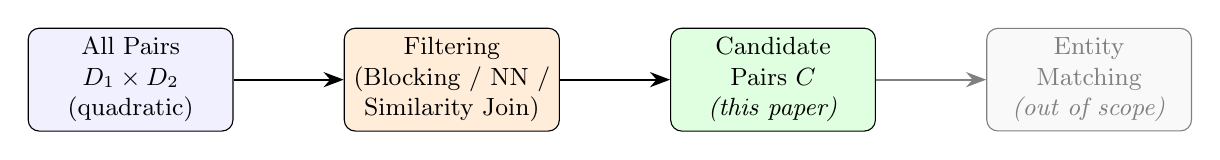
\begin{tikzpicture}[
  stage/.style={draw, rectangle, rounded corners, minimum width=2.6cm, minimum height=1.3cm, align=center, fill=blue!6, font=\small},
  arrow/.style={-{Stealth[scale=1.1]}, thick}
]
\node[stage] (all) {All Pairs\\$D_1 \times D_2$\\(quadratic)};
\node[stage, right=1.4cm of all, fill=orange!15] (filter) {Filtering\\(Blocking / NN /\\Similarity Join)};
\node[stage, right=1.4cm of filter, fill=green!12] (cand) {Candidate\\Pairs $C$\\\textit{(this paper)}};
\node[stage, right=1.4cm of cand, draw=gray, fill=gray!5, text=gray] (match) {Entity\\Matching\\\textit{(out of scope)}};
\draw[arrow] (all) -- (filter);
\draw[arrow] (filter) -- (cand);
\draw[arrow, gray] (cand) -- (match);
\end{tikzpicture}}
\caption{The Entity Resolution filtering pipeline. Filtering reduces all pairs to a much
smaller candidate set $C$, which the matching step then resolves into true duplicates.}
\label{fig:er-pipeline}
\end{figure}

Papadakis et al.~\cite{papadakis2023benchmarking} and, in extended journal form, Neuhof et al.~\cite{neuhof2024open} introduced the Continuous Filtering Benchmark, the first systematic comparison of \textit{blocking} and \textit{nearest-neighbor (NN) workflows}, the latter further split into \textit{sparse} syntactic methods (e.g., kNN-Join, $\varepsilon$-Join) and \textit{dense} learned-embedding methods (e.g., FAISS, ScaNN, DeepBlocker), across ten general-purpose datasets. We adopt this same taxonomy (Fig.~\ref{fig:taxonomy}).

\begin{figure}[!ht]
\centering
\resizebox{0.95\textwidth}{!}{%
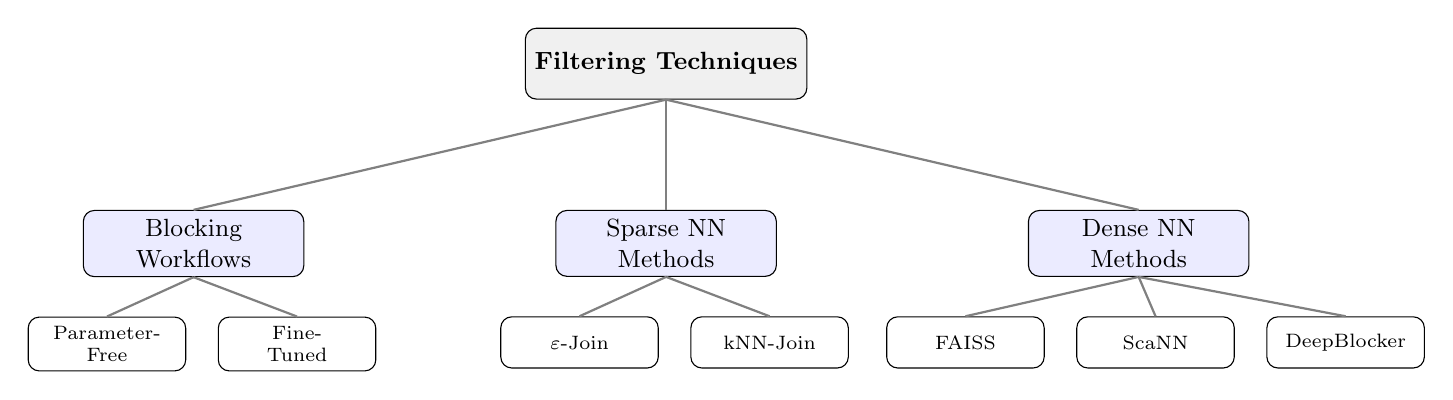
\begin{tikzpicture}[
  root/.style={draw, rectangle, rounded corners, minimum width=3.4cm, minimum height=0.9cm, align=center, fill=gray!12, font=\bfseries\small},
  fam/.style={draw, rectangle, rounded corners, minimum width=2.8cm, minimum height=0.8cm, align=center, font=\small, fill=blue!8},
  leaf/.style={draw, rectangle, rounded corners, minimum width=2.0cm, minimum height=0.65cm, align=center, font=\scriptsize},
  line/.style={-, thick, gray}
]
\node[root] (root) {Filtering Techniques};

\node[fam, below left=1.4cm and 2.8cm of root] (block) {Blocking\\Workflows};
\node[fam, below=1.4cm of root] (sparse) {Sparse NN\\Methods};
\node[fam, below right=1.4cm and 2.8cm of root] (dense) {Dense NN\\Methods};

\draw[line] (root.south) -- (block.north);
\draw[line] (root.south) -- (sparse.north);
\draw[line] (root.south) -- (dense.north);

\node[leaf, below=0.5cm of block, xshift=-1.1cm] (pf) {Parameter-\\Free};
\node[leaf, right=0.4cm of pf] (ft) {Fine-\\Tuned};
\draw[line] (block.south) -- (pf.north);
\draw[line] (block.south) -- (ft.north);

\node[leaf, below=0.5cm of sparse, xshift=-1.1cm] (eps) {$\varepsilon$-Join};
\node[leaf, right=0.4cm of eps] (knn) {kNN-Join};
\draw[line] (sparse.south) -- (eps.north);
\draw[line] (sparse.south) -- (knn.north);

\node[leaf, below=0.5cm of dense, xshift=-2.2cm] (faiss) {FAISS};
\node[leaf, right=0.4cm of faiss] (scann) {ScaNN};
\node[leaf, right=0.4cm of scann] (db) {DeepBlocker};
\draw[line] (dense.south) -- (faiss.north);
\draw[line] (dense.south) -- (scann.north);
\draw[line] (dense.south) -- (db.north);
\end{tikzpicture}}
\caption{Taxonomy of the three filtering families evaluated here, following the
blocking-vs.-nearest-neighbor split of Papadakis et al.~\cite{papadakis2023benchmarking} and
Neuhof et al.~\cite{neuhof2024open}, with nearest-neighbor methods split further into sparse
(syntactic) and dense (semantic) representations.}
\label{fig:taxonomy}
\end{figure}

This benchmark's findings, however, do not directly transfer to the medical domain, whose records exhibit properties that challenge standard filtering assumptions:
\begin{itemize}
    \item \textbf{Domain-specific vocabulary:} drug names, diagnosis codes, and anatomical terms are underrepresented in general-purpose language models, weakening pre-trained embeddings.
    \item \textbf{Short, homogeneous strings:} ontology datasets like UMLS contain short concept strings (e.g., ``Aspirin'' vs.\ ``Acetylsalicylic acid'') where non-matches overlap heavily and true matches may not, due to synonymy.
    \item \textbf{Scale and duplicate density:} datasets range from $\sim$800-record drug terminologies to ontology mappings of $\sim$135K$\times$157K records with 643K ground-truth pairs.
\end{itemize}

\noindent\textbf{Main Contributions}
\begin{enumerate}
    \item \textbf{A medical filtering benchmark:} to our knowledge, the first comprehensive
    evaluation of blocking, sparse NN, and dense NN filtering on nine medical ER datasets,
    establishing baselines for future research.
    \item \textbf{Parameter sensitivity:} fine-tuning blocking workflows yields gains of up to
    $70\times$ on Synthea and $6.6\times$ on CMS over parameter-free defaults, showing that
    one-size-fits-all configurations are inadequate for medical data.
    \item \textbf{Sparse vs.\ dense representations:} syntactic methods outperform
    general-purpose dense embeddings on seven of nine datasets, pointing to a
    domain-vocabulary gap in pre-trained sentence transformers.
    \item \textbf{A hard case:} UMLS resists every method, with no full-collection result
    above F\textsubscript{1}=0.31 and a reduced 50\% subset topping out at 0.53, owing to its
    scale, duplicate density, and short ontology terms.
    \item \textbf{Reproducibility findings:} implementation-level failure modes invisible in
    aggregate numbers, notably a tensor-shape mismatch in DeepBlocker's Hybrid model and a
    collapse of both approximate indices on CMS that exact search avoids.
\end{enumerate}

\section{Related Work}

\subsection{Entity Resolution and Filtering Techniques}
Entity Resolution (ER) has long been studied as record linkage, deduplication, or reference
reconciliation~\cite{christen2012datamatching}. Because pairwise comparison scales
quadratically, filtering (blocking) discards most non-matching pairs before any expensive
comparison~\cite{papadakis2021survey}. Classic methods build signatures from attribute values (tokens, character $n$-grams, sorted-neighborhood windows) and block entities sharing one. Meta-blocking~\cite{papadakis2014metablocking} then restructures these blocks into a weighted candidate-pair graph and prunes low-weight edges, via Weighted Edge Pruning, (Reciprocal) Cardinality Node Pruning, or the schema-aware BLAST algorithm~\cite{simonini2016blast}. With block purging and filtering, these form the \textit{blocking workflow} paradigm implemented in JedAI~\cite{papadakis2020jedai}, used throughout this work.

A separate line formulates filtering as a \textit{similarity join}: enumerate every pair whose similarity exceeds a threshold $\varepsilon$~\cite{mann2016setsimjoin}. Inverted-index joins ($\varepsilon$-Join) and their top-$k$ variant (kNN-Join) trade a tunable threshold for completeness guarantees under the chosen similarity function and representation.

\subsection{Nearest-Neighbor and Embedding-Based Methods for Entity Resolution}

Dense NN filtering embeds each entity as a fixed-length vector and retrieves candidates via
approximate nearest-neighbor search. FAISS~\cite{johnson2021billion} offers exact (flat) and
approximate graph-based (HNSW) search, trading a little recall for much faster queries.
ScaNN~\cite{guo2020scann} uses a learned tree partition and anisotropic quantization, exposing
the same brute-force-vs.-asymmetric-hashing trade-off. Both are agnostic to how vectors are
produced; following the base benchmark, we use general-purpose sentence embeddings
(all-MiniLM-L6-v2~\cite{reimers2019sentencebert}) rather than domain-specific ones.
DeepBlocker~\cite{thirumuruganathan2021deep} instead learns the tuple embedding itself, via an
unsupervised AutoEncoder, a self-supervised Cross-Tuple Training (CTT) objective, or a Hybrid
of both, before exact top-$k$ pairing.

\subsection{Benchmarking Filtering Techniques for Entity Resolution}

Blocking workflows and NN methods were rarely compared under a common protocol until
Papadakis et al.~\cite{papadakis2023benchmarking} and, in extended form, Neuhof et
al.~\cite{neuhof2024open}. Their Continuous Filtering Benchmark evaluates both families across
ten established ER datasets under schema-agnostic and schema-aware settings, reporting best
precision at fixed recall targets $\tau \in \{0.85, 0.90, 0.95\}$ rather than a single
operating point, since each technique's configuration space (filtering ratios, weighting
schemes, thresholds, $k$) has a first-order effect on the recall-precision trade-off. They
find that no paradigm dominates: blocking is most robust overall, sparse NN (kNN-Join)
overtakes it on long, clean textual attributes, and dense NN is consistently weakest,
penalized by the domain gap between general-purpose training corpora and dataset vocabulary.

We follow the same philosophy (parameter-free baselines, fine-tuned configurations, a common
harness) but apply it to the medical domain, absent from the original ten
bibliographic/e-commerce datasets, which we also use as a reproduction study
(Section~\ref{sec:results}) to validate our pipeline.

\subsection{Entity Resolution in the Medical and Biomedical Domain}
Medical ER spans patient-record deduplication, linking de-identified health records, and
aligning ontology concepts across vocabularies such as UMLS~\cite{bodenreider2004umls} and
RxNorm~\cite{nelson2011rxnorm}. Existing surveys~\cite{papadakis2021survey} address filtering
here only in passing.

On the patient-record side, filtering underpins privacy-preserving record linkage: Randall et
al.~\cite{randall2014pprl} scale inverted-index and sorted-neighborhood blocking to hospital
databases of millions of records, under encoding constraints our non-private methods avoid.
Febrl~\cite{christen2008febrl} was built for, and remains widely used in, health and census
linkage, akin to our FEBRL and Synthea~\cite{walonoski2018synthea} datasets.

On the ontology side, filtering overlaps with biomedical entity linking: mapping a mention to
its canonical UMLS concept, as in MedMentions~\cite{mohan2019medmentions}, is structurally
Clean-Clean ER. SapBERT~\cite{liu2021sapbert} learns dense embeddings aligned to UMLS synonym
clusters, unlike the general-purpose embeddings we evaluate; whether this closes the
sparse-over-dense gap we observe is left to future work. To our knowledge, ours is the first
systematic, multi-method quantification of how these medical-domain properties affect
filtering effectiveness.

\section{Medical Datasets}
\label{sec:datasets}

We assemble nine medical and biomedical ER datasets, summarized in Table~\ref{tab:datasets}, spanning three orders of magnitude in scale (500 to over 600K ground-truth pairs) and both major ER task formulations: \textit{Dirty ER}, where duplicates must be identified within a single, possibly noisy, collection ($D = D_1 = D_2$), and \textit{Clean-Clean ER}, where two internally clean collections must be linked against each other.

\begin{table}[!ht]
\centering
\caption{Overview of the nine medical datasets used in this benchmark.}
\label{tab:datasets}
\resizebox{\textwidth}{!}{%
\begin{tabular}{lllrrcc}
\toprule
\textbf{Dataset} & \textbf{Domain} & \textbf{Source} & \textbf{$|D_1|$} & \textbf{$|D_2|$} & \textbf{GT pairs} & \textbf{ER task} \\
\midrule
FEBRL-1     & Synthetic patient records     & Febrl generator~\cite{christen2008febrl} & 1,000   & 1,000   & 500     & Dirty ER \\
FEBRL-2     & Synthetic patient records     & Febrl generator~\cite{christen2008febrl} & 5,000   & 5,000   & 1,934   & Dirty ER \\
FEBRL-3     & Synthetic patient records     & Febrl generator~\cite{christen2008febrl} & 5,000   & 5,000   & 6,538   & Dirty ER \\
FEBRL-4     & Synthetic patient records     & Febrl generator~\cite{christen2008febrl} & 5,000   & 5,000   & 5,000   & Clean-Clean ER \\
Synthea     & Synthetic EHR patients        & Synthea generator~\cite{walonoski2018synthea} & 5,660   & 6,228   & 500     & Clean-Clean ER \\
MedMentions & PubMed entity mentions        & MedMentions corpus~\cite{mohan2019medmentions} & 22,248  & 22,248  & 22,248  & Clean-Clean ER \\
CMS         & Medicare physician records    & CMS Open Payments~\cite{cms2024openpayments} & 64,177  & 64,177  & 64,177  & Clean-Clean ER \\
UMLS        & Medical ontology concepts     & UMLS MRCONSO.RRF~\cite{bodenreider2004umls} & 134,992 & 156,932 & 643,166 & Clean-Clean ER \\
RxNorm      & Drug terminology (IN vs.\ BN) & NLM RxNorm CPC~\cite{nelson2011rxnorm} & 808     & 868     & 868     & Clean-Clean ER \\
\bottomrule
\end{tabular}}
\vspace{2pt}
\\ \footnotesize All collections are public: Febrl, Synthea and CMS need no registration,
MedMentions is CC0, and UMLS and RxNorm require a free NLM Metathesaurus License. Derived
collections, ground truth and preparation scripts are in our repository.
\end{table}

FEBRL-1 to FEBRL-3 are Dirty ER, with $D_1$ and $D_2$ the same file under increasing synthetic corruption: ground-truth pairs grow faster than the record count, so FEBRL-3 has 6{,}538 pairs among 5{,}000 records, indicating duplicate clusters larger than pairs. FEBRL-4 instead pairs two independently generated, clean 5{,}000-record populations with exactly one true match per record, making it Clean-Clean despite the shared family. Synthea likewise uses two populations: $D_1$ (5{,}660 records) unmodified, and $D_2$ (6{,}228 records) into which 500 noisy copies of $D_1$ records were injected as the ground truth. Despite this Dirty-ER-style noise injection, matches occur only across $D_1$ and $D_2$, never within either side, so Synthea is structurally Clean-Clean. The remaining four are Clean-Clean by construction: MedMentions links PubMed mention spans to their canonical concepts, CMS links two physician-record extracts, and UMLS and RxNorm link two source vocabularies, in each case with matches defined only across collections.

These datasets stress-test filtering along three axes underrepresented in general-purpose ER
benchmarks:
\begin{itemize}
    \item \textbf{Structured vs.\ unstructured records.} FEBRL and Synthea have fielded
    attributes (name, date of birth, address), whereas MedMentions consists of free-text
    mention spans, requiring schema-agnostic filtering.
    \item \textbf{Short, synonym-dense strings.} UMLS and RxNorm entities are often single or
    few-word concept names (drug ingredient vs.\ brand name), where token overlap between true
    matches can be low and between non-matches high.
    \item \textbf{Scale and duplicate density.} Inputs range from 808 records (RxNorm) to over
    150K (UMLS). UMLS's 643K ground-truth pairs exceed either collection, reflecting a
    many-to-many mapping, and are two orders of magnitude beyond any other dataset, a major
    driver of its difficulty (Section~\ref{sec:results}).
\end{itemize}

All datasets are processed under \textit{schema-agnostic} settings: filtering operates on the concatenation of all attribute values rather than a single distinguished attribute. This
follows Neuhof et al.~\cite{neuhof2024open} for their datasets with low schema-aware attribute coverage, and reflects MedMentions and UMLS, where no single attribute reliably identifies an entity across both sides of the match.


\section{Methodology}
\label{sec:methodology}

\subsection{Problem Definition and Evaluation Metrics}

Given two entity collections $D_1$ and $D_2$ (or a single collection $D$ for Dirty ER, treated
as $D_1 = D_2 = D$), a filtering technique produces candidate pairs $C \subseteq D_1 \times
D_2$ containing as many true duplicates (the ground truth $GT$) as possible, while keeping
$|C|$ small enough for subsequent pairwise matching to remain tractable. We report the standard
filtering-effectiveness measures:
\begin{equation}
PC = \frac{|C \cap GT|}{|GT|}, \qquad
PQ = \frac{|C \cap GT|}{|C|}, \qquad
F_1 = \frac{2 \cdot PC \cdot PQ}{PC + PQ}
\end{equation}
where $PC$ (Pair Completeness) is recall over the ground truth, $PQ$ (Pair Quality) is
precision over the candidate set, and $F_1$ their harmonic mean.

\subsection{Blocking Workflows}
\label{sec:methodology-blocking}

We evaluate two configurations of the JedAI blocking pipeline, both following the four-stage
workflow of block building, purging, filtering, and meta-blocking (comparison cleaning):
\begin{itemize}
    \item \textbf{Parameter-Free.} Standard Blocking for FEBRL, Synthea, MedMentions and CMS;
    Q-Grams Blocking ($q=6$) for UMLS and RxNorm, whose short concept strings yield degenerate
    token blocks. Comparison-based Block Purging removes oversized blocks (smoothing factor
    $1.0$) and Comparison Propagation removes redundant comparisons, requiring no
    dataset-specific tuning.
    \item \textbf{Fine-Tuned.} We grid-search block builders (Standard; Q-Grams,
    
    $q \in \{2,\ldots,6\}$), purging (on/off), block filtering ratios, and four meta-blocking
    algorithms (WEP, CEP, (Reciprocal) CNP, BLAST) with multiple edge-weighting schemes (ARCS,
    CBS, JS, EJS, PEARSON\_X2), matching the configuration space of the reproduction study in
    Section~\ref{sec:results}. We report the configuration maximizing $F_1$ directly, not the
    fixed-recall protocol ($PC \geq \tau$, $\tau \in \{0.85, 0.90, 0.95\}$) of the base
    benchmark; for CMS and UMLS, whose scale makes the full grid impractical, we search a
    reduced grid of 3 meta-blocking methods, 3 weighting schemes and 3 filtering ratios.
\end{itemize}

\subsection{Sparse Nearest-Neighbor Methods}
\textbf{$\varepsilon$-Join.} We implement a schema-agnostic inverted-index similarity join:
entities are tokenized, an index is built over the source collection, and for each target
entity, candidates sharing at least one token are scored by cosine or Jaccard similarity and
retained above a per-dataset threshold $\varepsilon$. Character trigrams are used for the
short, synonym-dense UMLS, RxNorm and MedMentions vocabularies, whitespace tokens elsewhere;
Table~\ref{tab:eps-join-config} lists the threshold, similarity and tokenizer per dataset.

\textbf{kNN-Join.} We additionally implement the top-$k$ variant, retrieving for each query
entity the $k$ candidates with highest token-based similarity (ties at the $k$th score
retained). We evaluate $k \in \{1,5,10,20,50,100\}$ and select the highest-$F_1$ configuration
per dataset. Tokenizers follow the same pattern as $\varepsilon$-Join; CMS uses Jaccard
similarity, the rest cosine. Table~\ref{tab:knn-join-medical} reports the selected $k$ and
effectiveness scores.

\subsection{Dense Nearest-Neighbor Methods}
All dense NN methods operate on 384-dimensional sentence embeddings from the pre-trained
\texttt{all-MiniLM-L6-v2} model~\cite{reimers2019sentencebert}, applied to the concatenated
attribute values of each entity, with no domain-specific fine-tuning.
\begin{itemize}
    \item \textbf{FAISS.} An exact \texttt{IndexFlatIP} (inner-product search over
    $L_2$-normalized vectors, equivalent to exact cosine search) and an approximate
    \texttt{IndexHNSWFlat} ($M=32$, $\mathit{ef\_construction}=200$), for
    $k \in \{1,5,10,20,50,100\}$.
    \item \textbf{ScaNN.} An asymmetric-hashing (AH) index using dot-product scoring on
    normalized vectors, with leaves and training sample size scaled to the collection
    (Section~\ref{sec:results-nn}).
    \item \textbf{DeepBlocker.} The AutoEncoder (unsupervised reconstruction), CTT
    (self-supervised Cross-Tuple Training) and Hybrid (concatenation of both) tuple-embedding
    variants, each with exact top-$k$ pairing, for $k \in \{1,5,10,50\}$.
\end{itemize}

\subsection{Experimental Environment}
Blocking and $\varepsilon$-/kNN-Join experiments run in Java on JedAI (\texttt{-Xmx12g} for
CMS and UMLS); dense NN experiments run in Python on a SLURM-managed GPU/CPU cluster. Since
the two differ in language and hardware, we follow the ANN-Benchmarks
methodology~\cite{aumuller2020annbenchmarks} of comparing \textit{implementations} rather than \textit{algorithms}, restricting cross-family run-time comparisons to relative orders of magnitude.


\section{Results}
\label{sec:results}

\subsection{Reproduction on General-Purpose Datasets}
\label{sec:results-reproduction}

Table~\ref{tab:baseline-blocking} and Table~\ref{tab:baseline-knnjoin} report our reproduction
of the blocking-workflow and kNN-Join baselines from the Continuous Filtering
Benchmark~\cite{papadakis2023benchmarking,neuhof2024open} on its original ten datasets, using
their published per-dataset configurations. The kNN-Join setup is notably heterogeneous: $k$
ranges from 1 on six datasets to 26 on Amazon-Google Products, and character $n$-gram size
varies from 2 to 5, evidence of the sparse family's sensitivity to tuning. Both tables match
the base benchmark's trends: high effectiveness on clean bibliographic data (F\textsubscript{1}
above 0.9 on DBLP-ACM and DBLP-Scholar) and sharp precision drops on noisy or many-to-one
vocabularies, where Amazon-Google Products needs $k=26$ to reach 0.900 recall and lands at
0.028 precision. This validates that our JedAI-based pipeline is correctly configured before
we apply it to medical data.

\begin{table}[!ht]
\centering
\caption{Blocking workflow reproduction on the ten general-purpose ER datasets. All use
Standard Blocking; BF is the block filtering ratio; purging is comparison-based, smoothing
factor 1.0. CNP = Cardinality Node Pruning, RCNP = Reciprocal CNP.}
\label{tab:baseline-blocking}
\resizebox{\textwidth}{!}{%
\begin{tabular}{lcccccc}
\toprule
\textbf{Dataset} & \textbf{Purging} & \textbf{BF} & \textbf{Meta-blocking (weighting)} & \textbf{PC} & \textbf{PQ} & \textbf{F\textsubscript{1}} \\
\midrule
Restaurant       & no  & 0.050 & WEP (ARCS)          & 1.000 & 0.533 & 0.695 \\
Abt-Buy          & no  & 0.875 & BLAST (PEARSON\_X2) & 0.902 & 0.216 & 0.349 \\
Amazon-GP        & yes & 0.925 & CNP (PEARSON\_X2)   & 0.901 & 0.017 & 0.033 \\
DBLP-ACM         & yes & 0.225 & RCNP (EJS)          & 0.903 & 0.957 & 0.929 \\
IMDb-TMDb        & yes & 1.000 & RCNP (CBS)          & 0.922 & 0.382 & 0.540 \\
IMDb-TVDb        & no  & 0.975 & RCNP (CBS)          & 0.924 & 0.189 & 0.314 \\
TMDb-TVDb        & no  & 0.350 & RCNP (CBS)          & 0.909 & 0.154 & 0.264 \\
Walmart-Amazon   & no  & 0.225 & RCNP (ARCS)         & 0.904 & 0.117 & 0.207 \\
DBLP-Scholar     & yes & 0.625 & RCNP (JS)           & 0.915 & 0.470 & 0.621 \\
IMDb-DBpedia     & no  & 0.800 & BLAST (PEARSON\_X2) & 0.904 & 0.475 & 0.623 \\
\bottomrule
\end{tabular}}
\end{table}

\begin{table}[!ht]
\centering
\caption{kNN-Join reproduction on the ten general-purpose ER datasets, using the base
benchmark's per-dataset configuration. $k$ is per target-collection query entity.}
\label{tab:baseline-knnjoin}
\resizebox{0.8\textwidth}{!}{%
\begin{tabular}{llccccc}
\toprule
\textbf{Dataset} & \textbf{Tokenizer} & \textbf{Similarity} & \textbf{$k$} & \textbf{PC} & \textbf{PQ} & \textbf{F\textsubscript{1}} \\
\midrule
Restaurant       & Char 4-grams (multiset) & Dice   & 1  & 1.000 & 0.224 & 0.366 \\
Abt-Buy          & Char 3-grams (multiset) & Cosine & 4  & 0.924 & 0.229 & 0.367 \\
Amazon-GP        & Char 5-grams (multiset) & Cosine & 26 & 0.900 & 0.028 & 0.055 \\
DBLP-ACM         & Char 2-grams (multiset) & Cosine & 1  & 0.996 & 0.954 & 0.974 \\
IMDb-TMDb        & Char 5-grams            & Cosine & 1  & 0.961 & 0.305 & 0.463 \\
IMDb-TVDb        & Char 5-grams            & Cosine & 1  & 0.910 & 0.122 & 0.215 \\
TMDb-TVDb        & Char 5-grams            & Cosine & 1  & 0.972 & 0.130 & 0.229 \\
Walmart-Amazon   & Char 4-grams (multiset) & Cosine & 2  & 0.910 & 0.150 & 0.258 \\
DBLP-Scholar     & Char 4-grams            & Cosine & 1  & 0.957 & 0.877 & 0.915 \\
IMDb-DBpedia     & Char 4-grams            & Cosine & 5  & 0.903 & 0.149 & 0.256 \\
\bottomrule
\end{tabular}}
\end{table}

\subsection{Blocking Workflows on Medical Data}
\label{sec:results-blocking}
Table~\ref{tab:medical-blocking} reports the parameter-free and fine-tuned blocking workflows
on all nine medical datasets. The parameter-free workflow alone exposes a clear pattern: it is
competitive when attribute values are long and low-noise (FEBRL-4 at 0.907, MedMentions at
0.949), and collapses on the more heavily corrupted FEBRL-2 and FEBRL-3, and on UMLS, where
Q-Gram blocks are simultaneously too small for adequate recall and too numerous for adequate
precision. RxNorm underperforms differently: recall is high (PC=0.931) but precision only
0.075, because a single active ingredient generates many surface forms sharing Q-Grams with
unrelated products.

\begin{table}[!ht]
\centering
\caption{Blocking workflows on medical datasets: parameter-free (PF) vs.\ fine-tuned (FT),
with the best grid-search configuration. BF = block filtering ratio, WEP = Weighted Edge
Pruning, RCNP = Reciprocal Cardinality Node Pruning.}
\label{tab:medical-blocking}
\resizebox{\textwidth}{!}{%
\begin{tabular}{lccccccc}
\toprule
& & \multicolumn{3}{c}{\textbf{Parameter-free}} & \multicolumn{3}{c}{\textbf{Fine-tuned}} \\
\cmidrule(lr){3-5}\cmidrule(lr){6-8}
\textbf{Dataset} & \textbf{Best FT configuration}
                 & \textbf{PC} & \textbf{PQ} & \textbf{F\textsubscript{1}}
                 & \textbf{PC} & \textbf{PQ} & \textbf{F\textsubscript{1}} \\
\midrule
FEBRL-1     & Standard, BF=0.30, WEP                    & 1.000 & 0.240 & 0.387 & 0.998 & 0.250 & 0.400 \\
FEBRL-2     & Q-Grams ($q$=4), BF=0.35, BLAST           & 0.116 & 0.026 & 0.043 & 0.511 & 0.112 & 0.184 \\
FEBRL-3     & Q-Grams ($q$=4), BF=0.35, BLAST           & 0.103 & 0.102 & 0.102 & 0.451 & 0.166 & 0.242 \\
FEBRL-4     & Standard, BF=0.20, BLAST                  & 0.993 & 0.835 & 0.907 & 1.000 & 1.000 & 1.000 \\
Synthea     & Standard, purging, BF=0.10, WEP           & 1.000 & 0.007 & 0.014 & 0.986 & 0.978 & 0.982 \\
MedMentions & Standard, purging, BF=0.35, RCNP          & 1.000 & 0.903 & 0.949 & 1.000 & 0.994 & 0.997 \\
CMS         & Standard, BF=0.20, RCNP$^{*}$             & 0.901 & 0.077 & 0.141 & 0.966 & 0.888 & 0.925 \\
UMLS        & Q-Grams ($q$=6), purging, BF=0.10, RCNP$^{*}$ & 0.155 & 0.001 & 0.002 & 0.134 & 0.338 & 0.191 \\
RxNorm      & Q-Grams ($q$=5), BF=0.35, BLAST           & 0.931 & 0.075 & 0.139 & 0.909 & 0.822 & 0.863 \\
\bottomrule
\end{tabular}}
\vspace{2pt}
\\ \footnotesize $^{*}$ Reduced grid (3 meta-blocking methods, 3 weighting schemes, 3 BF
settings); the full grid was terminated.
\end{table}

Fine-tuning improves every dataset, transformatively on three: Synthea by $70\times$, CMS by
$6.6\times$ and RxNorm by $6.2\times$. Once tuned, even tasks with very small ground truth
relative to search space (Synthea: 500 pairs against 11{,}888 profiles) can be filtered almost perfectly. Two datasets resist tuning: FEBRL-1 moves only from 0.387 to 0.400, UMLS reaches only 0.191. In both, block-building is the bottleneck: no grid setting makes corrupted or synonymous profiles reliably co-occur, leaving downstream pruning ineffective. This is the first departure from the base benchmark, where tuned blocking workflows are consistently strongest.

The PC columns qualify this. On UMLS, RxNorm and Synthea, fine-tuning raises
F\textsubscript{1} partly by trading recall away (UMLS PC falls from 0.155 to 0.134). Because filtering recall bounds the recall of the whole ER pipeline, an F\textsubscript{1}-maximizing grid search can select configurations that a deployed system would reject, which is precisely what the base benchmark's fixed-recall protocol ($PC \geq \tau$) is designed to avoid.

\subsection{Sparse Nearest-Neighbor Methods: $\varepsilon$-Join and kNN-Join}
\label{sec:results-sparse}

Unlike blocking, $\varepsilon$-Join requires no meta-blocking stage, trading a smaller
configuration space for less flexibility in the precision-recall trade-off. Its behavior is
strongly bimodal. On the FEBRL family it runs high-recall and low-precision (PC above 0.94,
PQ between 0.21 and 0.36), whereas on MedMentions, CMS and UMLS it inverts, reaching precision
of 0.99 or higher while retrieving under a fifth of true matches on the latter two. CMS is
clearest: at $\varepsilon = 0.70$ all 6{,}287 retained pairs are correct, but 90\% of the
ground truth never enters the candidate set. A single global threshold cannot serve both
regimes, the method's central limitation here.

\begin{table}[!ht]
\centering
\caption{$\varepsilon$-Join on medical datasets, with per-dataset configuration.}
\label{tab:eps-join-config}
\resizebox{\textwidth}{!}{%
\begin{tabular}{lcccccc}
\toprule
\textbf{Dataset} & \textbf{Tokenizer} & \textbf{Similarity} & \textbf{$\varepsilon$} & \textbf{PC} & \textbf{PQ} & \textbf{F\textsubscript{1}} \\
\midrule
FEBRL-1      & Whitespace         & Cosine  & 0.50 & 0.996 & 0.250 & 0.399 \\
FEBRL-2      & Whitespace         & Cosine  & 0.50 & 0.958 & 0.213 & 0.348 \\
FEBRL-3      & Whitespace         & Cosine  & 0.50 & 0.946 & 0.356 & 0.517 \\
FEBRL-4      & Whitespace         & Cosine  & 0.50 & 0.994 & 1.000 & 0.997 \\
Synthea      & Whitespace         & Cosine  & 0.40 & 1.000 & 0.026 & 0.051 \\
MedMentions  & Character trigrams & Cosine  & 0.60 & 0.573 & 0.986 & 0.725 \\
CMS          & Whitespace         & Jaccard & 0.70 & 0.098 & 1.000 & 0.178 \\
UMLS         & Character trigrams & Cosine  & 0.60 & 0.185 & 0.925 & 0.308 \\
RxNorm       & Character trigrams & Cosine  & 0.50 & 0.624 & 0.221 & 0.327 \\
\bottomrule
\end{tabular}}
\end{table}

\begin{table}[!ht]
\centering
\caption{kNN-Join on medical datasets. The selected value of $k$ maximizes F\textsubscript{1}
over $k \in \{1,5,10,20,50,100\}$. UMLS results use the ground-truth-complete 50\% subset.}
\label{tab:knn-join-medical}
\resizebox{\textwidth}{!}{%
\begin{tabular}{lcccccc}
\toprule
\textbf{Dataset} & \textbf{Tokenizer} & \textbf{Similarity} & \textbf{$k$} & \textbf{PC} & \textbf{PQ} & \textbf{F\textsubscript{1}} \\
\midrule
FEBRL-1            & Whitespace         & Cosine  & 1 & 1.000 & 1.000 & 1.000 \\
FEBRL-2            & Whitespace         & Cosine  & 1 & 0.590 & 0.169 & 0.263 \\
FEBRL-3            & Whitespace         & Cosine  & 1 & 0.533 & 0.671 & 0.594 \\
FEBRL-4            & Whitespace         & Cosine  & 1 & 1.000 & 1.000 & 1.000 \\
Synthea            & Whitespace         & Cosine  & 1 & 1.000 & 0.079 & 0.146 \\
MedMentions        & Character trigrams & Cosine  & 1 & 0.940 & 0.938 & 0.939 \\
CMS                & Whitespace         & Jaccard & 1 & 0.962 & 0.665 & 0.787 \\
UMLS (50\% subset) & Character trigrams & Cosine  & 5 & 0.552 & 0.512 & 0.531 \\
RxNorm             & Character trigrams & Cosine  & 1 & 0.812 & 0.864 & 0.837 \\
\bottomrule
\end{tabular}}
\end{table}

kNN-Join varies the neighbors retained per query entity, and
Table~\ref{tab:knn-join-medical} shows that $k=1$ maximizes F\textsubscript{1} on eight of nine
datasets, as increasing $k$ preserves or improves PC while reducing PQ roughly proportionally.
The exception is the 50\% UMLS subset, where raising $k$ from 1 to 5 lifts PC from 0.202 to
0.552 at a small enough precision cost to yield the best observed F\textsubscript{1} of 0.531.
This is the signature of a dataset where the correct match often ranks second or third, as
expected when one concept has many near-equivalent surface forms competing for the top
position. kNN-Join is perfect on FEBRL-1 and FEBRL-4 and strong on MedMentions, RxNorm and CMS,
but weaker on the noisier FEBRL-2 and FEBRL-3.

\subsection{Dense Nearest-Neighbor Methods: FAISS, ScaNN, and DeepBlocker}
\label{sec:results-nn}

Table~\ref{tab:dense-nn} reports the best F\textsubscript{1} achieved by FAISS (Flat and HNSW)
and ScaNN (AH) on each medical dataset. Unlike the general-purpose setting, approximation is
not uniformly cheap here. HNSW stays within two points of Flat on seven of the nine datasets,
but on CMS it collapses from 0.859 to 0.309, and ScaNN's asymmetric hashing collapses the same
way to 0.288. This is not a retrieval-budget effect: HNSW recall on CMS is 0.309 at $k=1$ and
still only 0.375 at $k=100$, so a larger candidate set does not recover the missing matches.
Two independently implemented indices saturating at nearly the same recall points to the
embedding geometry rather than either index: CMS profiles are short physician-name strings
whose sentence embeddings cluster too tightly for the HNSW proximity graph or ScaNN's
anisotropic partitioning to separate locally. The choice of index is therefore not orthogonal to effectiveness on medical data, and the penalty falls on CMS, the dataset where the approximate variants are otherwise most attractive.

\begin{table}[!ht]
\centering
\caption{Dense NN best F\textsubscript{1} per medical dataset over
$k \in \{1,5,10,20,50,100\}$, using 384-dimensional \texttt{all-MiniLM-L6-v2} embeddings.
F\textsubscript{1} decreases monotonically in $k$ beyond $k^{*}$. Only F\textsubscript{1} is
shown: at $k^{*}=1$ on the datasets where $|D_1| = |D_2| = |GT|$ each query returns exactly one
candidate, so PC = PQ = F\textsubscript{1} by construction.}
\label{tab:dense-nn}
\begin{tabular}{lcccc}
\toprule
\textbf{Dataset} & \textbf{$k^{*}$} & \textbf{FAISS Flat} & \textbf{FAISS HNSW} & \textbf{ScaNN AH} \\
\midrule
FEBRL-1      & 1 & 0.955 & 0.955 & 0.819 \\
FEBRL-2      & 1 & 0.315 & 0.315 & 0.285 \\
FEBRL-3      & 1 & 0.551 & 0.550 & 0.497 \\
FEBRL-4      & 1 & 0.931 & 0.917 & 0.730 \\
Synthea      & 1 & 0.162 & 0.160 & 0.159 \\
MedMentions  & 1 & 0.656 & 0.637 & 0.569 \\
CMS          & 1 & 0.859 & 0.309 & 0.288 \\
UMLS$^{*}$   & 5 & 0.415 & 0.410 & 0.399 \\
RxNorm       & 1 & 0.597 & 0.594 & 0.547 \\
\bottomrule
\end{tabular}
\vspace{2pt}
\\ \footnotesize $^{*}$ UMLS values come from a separate run on the full collections; the other
eight rows use the run described in Section~\ref{sec:methodology}.
\end{table}

DeepBlocker's medical evaluation is incomplete and its precision measurements unusable, so we
report it separately in Table~\ref{tab:deepblocker} as a qualitative, recall-focused data point
rather than a comparable F\textsubscript{1} score:
\begin{itemize}
    \item The \texttt{candidates} field is logged as $0.0$ in every run, forcing precision (PQ)
    to $0.0$ even where recall is high. We therefore report only the best recall (PC) per
    dataset, marked $\ddagger$ throughout.
    \item The \textbf{Hybrid} variant fails on \textit{every} dataset with an identical matrix-shape error (\texttt{mat1 and mat2 shapes cannot be multiplied 
    (256x150, 300x300)}), indicating a fixed embedding-dimension mismatch rather than a data-specific issue. It is omitted from Table~\ref{tab:deepblocker}.
    \item The run terminated during MedMentions, after AutoEncoder had completed all $k$ but
    before CTT began, leaving the result file marked \texttt{.partial} and CMS and UMLS with no
    results. CTT is roughly eight times slower than AutoEncoder on the smaller collections,
    which points to a resource limit on the 22{,}248-profile MedMentions run.
\end{itemize}

\begin{table}[!ht]
\centering
\caption{DeepBlocker best recall (PC$\ddagger$) per dataset and variant; precision is
unavailable (see text). PC is non-decreasing in $k$, so the reported $k$ is the smallest
attaining the maximum over $k \in \{1,5,10,50\}$, unlike the F\textsubscript{1}-maximizing $k$
elsewhere. ``--'' marks no result.}
\label{tab:deepblocker}
\begin{tabular}{lcccc}
\toprule
\textbf{Dataset} & \textbf{AE $k$} & \textbf{AE PC} & \textbf{CTT $k$} & \textbf{CTT PC} \\
\midrule
FEBRL-1      & 5  & 1.000 & 10 & 1.000 \\
FEBRL-2      & 50 & 0.997 & 50 & 0.999 \\
FEBRL-3      & 50 & 0.996 & 50 & 0.997 \\
FEBRL-4      & 50 & 0.998 & 50 & 0.999 \\
Synthea      & 1  & 1.000 & 1  & 1.000 \\
MedMentions  & 50 & 0.556 & \textit{--} & \textit{--} \\
CMS          & \textit{--} & \textit{--} & \textit{--} & \textit{--} \\
UMLS         & \textit{--} & \textit{--} & \textit{--} & \textit{--} \\
RxNorm       & 50 & 0.910 & 50 & 0.911 \\
\bottomrule
\end{tabular}
\end{table}

\section{Discussion}
\label{sec:discussion}

Table~\ref{tab:cross-family} consolidates the best result per dataset and method family.

\begin{table}[!ht]
\centering
\caption{Best $F_1$ per dataset and method family; per-metric values are in
Tables~\ref{tab:medical-blocking} to~\ref{tab:dense-nn}. FAISS entries are the better of Flat
and HNSW (Flat except on Synthea); dense and kNN-Join entries are at $k^{*}$; DeepBlocker
entries are best PC (marked $\ddagger$), since PQ is unavailable
(Table~\ref{tab:deepblocker}). Bold marks the best comparable $F_1$ per row.}
\label{tab:cross-family}
\resizebox{\textwidth}{!}{%
\begin{tabular}{lccccccc}
\toprule
\textbf{Dataset} & \textbf{Block.\ (PF)} & \textbf{Block.\ (FT)} & \textbf{$\varepsilon$-Join} & \textbf{kNN-Join} & \textbf{FAISS} & \textbf{ScaNN} & \textbf{DeepBlocker (PC)} \\
\midrule
FEBRL-1      & 0.387 & 0.400 & 0.399 & \textbf{1.000} & 0.955 & 0.819 & 1.000$\ddagger$ \\
FEBRL-2      & 0.043 & 0.184 & \textbf{0.348} & 0.263 & 0.315 & 0.285 & 0.999$\ddagger$ \\
FEBRL-3      & 0.102 & 0.242 & 0.517 & \textbf{0.594} & 0.551 & 0.497 & 0.997$\ddagger$ \\
FEBRL-4      & 0.907 & \textbf{1.000} & 0.997 & \textbf{1.000} & 0.931 & 0.730 & 0.999$\ddagger$ \\
Synthea      & 0.014 & \textbf{0.982} & 0.051 & 0.146 & 0.162 & 0.159 & 1.000$\ddagger$ \\
MedMentions  & 0.949 & \textbf{0.997} & 0.725 & 0.939 & 0.656 & 0.569 & 0.556$\ddagger$ \\
CMS          & 0.141 & \textbf{0.925} & 0.178 & 0.787 & 0.859 & 0.288 & not reached \\
UMLS         & 0.002 & 0.191 & 0.308 & \textbf{0.531} & 0.415 & 0.399 & not reached \\
RxNorm       & 0.139 & \textbf{0.863} & 0.327 & 0.837 & 0.597 & 0.547 & 0.911$\ddagger$ \\
\bottomrule
\end{tabular}}
\vspace{2pt}
\\ \footnotesize (i) All UMLS entries use the full collections except kNN-Join, run on a
ground-truth-complete 50\% subset ($|D_1|=67{,}188$, $|D_2|=78{,}466$, 323{,}550 pairs).
(ii) Synthea was regenerated between the blocking and $\varepsilon$-Join runs
($|D_2|=6{,}228$) and the nearest-neighbor runs ($|D_2|=8{,}026$); the 500 ground-truth pairs
are unchanged, but the roughly 30\% smaller search space slightly favors the former in PQ.
\end{table}

\textbf{No single filtering paradigm dominates.} As in the base
benchmark~\cite{papadakis2023benchmarking,neuhof2024open}, the best family is dataset-dependent
even within one domain. Fine-tuned blocking, $\varepsilon$-Join and kNN-Join each take at least
one dataset outright: blocking leads on Synthea, MedMentions, CMS and RxNorm and ties FEBRL-4;
kNN-Join at $k=1$ leads on FEBRL-1, FEBRL-3 and UMLS; $\varepsilon$-Join on FEBRL-2. A medical
ER pipeline therefore cannot select a filtering family a priori from general-purpose results,
which argues for either an ensemble of filters or a lightweight per-dataset selection step.

\textbf{Fine-tuning is necessary but not sufficient.} It improves blocking on all nine
datasets, and the $70\times$ gain on Synthea and $6.6\times$ on CMS dwarf the differences
between families: for a fixed engineering budget, configuration search on one well-understood
method is often worth more than adding untuned families. Yet the tuned workflow matches or
exceeds every other family on only five datasets. On the three dirty FEBRL variants and on UMLS
it is beaten, on FEBRL-1 decisively, by kNN-Join. This qualifies rather than contradicts the
base benchmark's finding that tuned blocking is most robust: blocking loses where attribute
values are short and character-corrupted, so no grid point yields blocks both small enough for
precision and large enough for recall.

\textbf{Sparse representations outperform dense ones on seven of nine datasets.} Dense
retrieval wins outright only on CMS, whose near-1-to-1 physician-name structure suits fixed-$k$
retrieval and whose name variants embeddings capture better than Jaccard tokenization, and
marginally on Synthea, where both families are weak. This mirrors the explanation Neuhof et
al.~\cite{neuhof2024open} give for general-purpose data: all-MiniLM-L6-v2 is trained on web and
news text, so medical terminology is underrepresented and embedding similarity is a noisier
proxy for duplication than character overlap. The sharpest evidence is internal to the sparse
family. On RxNorm, $\varepsilon$-Join and kNN-Join use identical character-trigram
representations yet score 0.327 and 0.837, so the gap is attributable to the retrieval rule,
not the representation: a single global threshold cannot serve a vocabulary in which ingredient
and brand names vary widely in length, whereas fixed-$k$ retrieval adapts per entity.
Confirming the domain-vocabulary hypothesis would require a domain-specific embedding baseline
(BioBERT, SapBERT), which we did not run.

\textbf{UMLS is hard for every method.} The best result is kNN-Join's $F_1=0.531$ on the 50\%
subset; on the full collections nothing exceeds 0.415. UMLS compounds three difficulties from
Section~\ref{sec:datasets}: scale ($134{,}992 \times 156{,}932$), many-to-many concept mapping
(643{,}166 pairs), and short synonym-dense strings. We regard UMLS-scale
ontology matching as future work rather than a case general-purpose filtering can be expected
to solve.

\textbf{DeepBlocker needs engineering hardening before fair comparison.} The uniform
\texttt{candidates=0} defect, the deterministic Hybrid failure, and the run terminating during
MedMentions make our numbers a lower bound rather than an assessment. This matches the base
benchmark's observation that learned tuple embeddings are harder to configure than sparse
counterparts, because stochastic components make failures less visible than a miscalibrated
threshold.

\textbf{Limitations.} We evaluate only schema-agnostic settings, though the base benchmark shows
schema-aware settings can change which family wins, and all dense methods use a single
general-purpose embedding model. Synthea's duplicates are generated by deleting one character from a single name attribute,
leaving all other fields identical, so every method attains near-perfect recall there and the
low F\textsubscript{1} values of the untuned methods reflect precision alone; it should not be
read as a hard corruption test. Finally, the
two comparability caveats under Table~\ref{tab:cross-family} mean the UMLS and Synthea rows are
not strictly like-for-like, and DeepBlocker remains incomplete on CMS and UMLS.


\section{Conclusion}
\label{sec:conclusion}
We extended the Continuous Filtering Benchmark to the medical domain, evaluating blocking
workflows (parameter-free and fine-tuned), sparse nearest-neighbor methods
($\varepsilon$-Join, kNN-Join) and dense ones (FAISS, ScaNN, DeepBlocker) across nine datasets
spanning synthetic patient records, electronic health records, biomedical text mentions and
medical ontologies, after first validating our JedAI-based pipeline on the benchmark's original
ten general-purpose datasets.

No single filtering family dominates. Fine-tuning yields larger gains than switching families,
$70\times$ in $F_1$ on Synthea and $6.6\times$ on CMS, and syntactic token-based methods
generally outperform general-purpose dense embeddings on medical vocabulary. Within the sparse
family, the retrieval rule matters as much as the representation: on RxNorm, $\varepsilon$-Join
and kNN-Join share a tokenizer yet score 0.327 and 0.837. On the full collections UMLS is the
hardest case, combining scale, duplicate density and short synonym-dense strings. We also
surfaced implementation issues invisible from aggregate numbers: a candidate-count logging
defect and a deterministic Hybrid-model failure in DeepBlocker, and a collapse of both
approximate indices on CMS that exact search does not share.

\textbf{Future work.} We plan to (1)~re-run the comparison at fixed recall thresholds
$\tau \in \{0.85, 0.90, 0.95\}$, following the base benchmark's protocol, since our PC columns
already show that $F_1$-maximizing configurations can trade recall away; (2)~fix the
DeepBlocker logging defect and Hybrid dimension mismatch and complete its evaluation on CMS and
UMLS; (3)~evaluate domain-specific biomedical embeddings (BioBERT, SapBERT) in place of
all-MiniLM-L6-v2, to test whether the sparse-over-dense gap reflects vocabulary coverage rather
than the dense paradigm itself; and (4)~extend to schema-aware settings, where a single
distinctive attribute (e.g., drug name in RxNorm) may change the ranking, as it does on
general-purpose datasets.
%
% , - Bibliography , -
%
\bibliographystyle{splncs04}
\begin{thebibliography}{21}

\bibitem{papadakis2023benchmarking}
Papadakis, G., Fisichella, M., Schoger, F., Mandilaras, G., Augsten, N., Nejdl, W.: Benchmarking filtering techniques for entity resolution. In: Proceedings of the 39th IEEE International Conference on Data Engineering (ICDE), pp.~653--666 (2023)

\bibitem{neuhof2024open}
Neuhof, F., Fisichella, M., Papadakis, G., Nikoletos, K., Augsten, N., Nejdl, W., Koubarakis, M.: Open benchmark for filtering techniques in entity resolution. The VLDB Journal \textbf{33}(5), 1671--1696 (2024)

\bibitem{christen2012datamatching}
Christen, P.: Data Matching: Concepts and Techniques for Record Linkage, Entity Resolution, and Duplicate Detection. Springer (2012)

\bibitem{papadakis2021survey}
Papadakis, G., Skoutas, D., Thanos, E., Palpanas, T.: Blocking and filtering techniques for entity resolution: a survey. ACM Computing Surveys \textbf{53}(2), 31:1--31:42 (2021)

\bibitem{papadakis2014metablocking}
Papadakis, G., Koutrika, G., Palpanas, T., Nejdl, W.: Meta-blocking: taking entity resolution to the next level. IEEE Transactions on Knowledge and Data Engineering \textbf{26}(8), 1946--1960 (2014)

\bibitem{simonini2016blast}
Simonini, G., Bergamaschi, S., Jagadish, H.V.: BLAST: a loosely schema-aware meta-blocking approach for entity resolution. Proceedings of the VLDB Endowment \textbf{9}(12), 1173--1184 (2016)

\bibitem{papadakis2020jedai}
Papadakis, G., Mandilaras, G.M., Gagliardelli, L., Simonini, G., Thanos, E., Giannakopoulos, G., Bergamaschi, S., Palpanas, T., Koubarakis, M.: Three-dimensional entity resolution with JedAI. Information Systems \textbf{93}, 101565 (2020)

\bibitem{randall2014pprl}
Randall, S.M., Ferrante, A.M., Boyd, J.H., Semmens, J.B.: Privacy-preserving record linkage on large real world datasets. Journal of Biomedical Informatics \textbf{50}, 205--212 (2014)

\bibitem{liu2021sapbert}
Liu, F., Shareghi, E., Meng, Z., Basaldella, M., Collier, N.: Self-alignment pretraining for biomedical entity representations. In: Proceedings of the 2021 Conference of the North American Chapter of the Association for Computational Linguistics: Human Language Technologies (NAACL-HLT), pp.~4228--4238 (2021)

\bibitem{mann2016setsimjoin}
Mann, W., Augsten, N., Bouros, P.: An empirical evaluation of set similarity join techniques. Proceedings of the VLDB Endowment \textbf{9}(9), 636--647 (2016)

\bibitem{johnson2021billion}
Johnson, J., Douze, M., J\'egou, H.: Billion-scale similarity search with GPUs. IEEE Transactions on Big Data \textbf{7}(3), 535--547 (2021)

\bibitem{guo2020scann}
Guo, R., Sun, P., Lindgren, E., Geng, Q., Simcha, D., Chern, F., Kumar, S.: Accelerating large-scale inference with anisotropic vector quantization. In: Proceedings of the 37th International Conference on Machine Learning (ICML) (2020)

\bibitem{thirumuruganathan2021deep}
Thirumuruganathan, S., Li, H., Tang, N., Ouzzani, M., Govind, Y., Paulsen, D., Fung, G., Doan, A.: Deep learning for blocking in entity matching: a design space exploration. Proceedings of the VLDB Endowment \textbf{14}(11), 2459--2472 (2021)

\bibitem{reimers2019sentencebert}
Reimers, N., Gurevych, I.: Sentence-BERT: sentence embeddings using Siamese BERT-networks. In: Proceedings of the 2019 Conference on Empirical Methods in Natural Language Processing (EMNLP-IJCNLP), pp.~3982--3992 (2019)

\bibitem{christen2008febrl}
Christen, P.: Febrl -- a freely available record linkage system with a graphical user interface. In: Proceedings of the 2nd Australasian Workshop on Health Data and Knowledge Management, pp.~17--25 (2008)

\bibitem{mohan2019medmentions}
Mohan, S., Li, D.: MedMentions: a large biomedical corpus annotated with UMLS concepts. In: Proceedings of the Automated Knowledge Base Construction Conference (AKBC) (2019)

\bibitem{cms2024openpayments}
Centers for Medicare \& Medicaid Services: Open Payments Data.
\url{https://openpaymentsdata.cms.gov/}, accessed 2026-08-27

\bibitem{aumuller2020annbenchmarks}
Aum\"uller, M., Bernhardsson, E., Faithfull, A.: ANN-Benchmarks: a benchmarking tool for approximate nearest neighbor algorithms. Information Systems \textbf{87}, 101374 (2020)

\bibitem{bodenreider2004umls}
Bodenreider, O.: The Unified Medical Language System (UMLS): integrating biomedical terminology. Nucleic Acids Research \textbf{32}(suppl\_1), D267--D270 (2004)

\bibitem{walonoski2018synthea}
Walonoski, J., Kramer, M., Nichols, J., Quina, A., Moesel, C., Hall, D., Duffett, C., Dube, K., Gallagher, T., McLachlan, S.: Synthea: an approach, method, and software mechanism for generating synthetic patients and the synthetic electronic health care record. Journal of the American Medical Informatics Association \textbf{25}(3), 230--238 (2018)

\bibitem{nelson2011rxnorm}
Nelson, S.J., Zeng, K., Kilbourne, J., Powell, T., Moore, R.: Normalized names for clinical drugs: RxNorm at 6 years. Journal of the American Medical Informatics Association \textbf{18}(4), 441--448 (2011)

\end{thebibliography}
\end{document}